

\newcommand{\beginsupplement}{%
        \setcounter{table}{0}
        %\renewcommand{\tablename}{S}%
        \renewcommand{\thetable}{S\arabic{table}}%
        \setcounter{algorithm}{0}
        %\renewcommand{\tablename}{S}%
        \renewcommand{\thealgorithm}{S\arabic{algorithm}}%
        \setcounter{equation}{0}
        %\renewcommand{\tablename}{S}%
        \renewcommand{\theequation}{S\arabic{equation}}%
        \setcounter{figure}{0}
        %\renewcommand{\figurename}{\textbf{Extended Data Fig.}}%
        \renewcommand{\thefigure}{S\arabic{figure}}%
        \setcounter{section}{0}
        \renewcommand{\thesection}{S\arabic{section}}%
     }

\beginsupplement

\section{Appendix\\ {\large Proofs of the Theorems}}
\begin{lemma}[Stochastic lower bound $F_{L,\gamma}$]\label{app_lemma:F_L}
    Consider the experiment of randomly sampling two times $m$ points of the initial ball $\calB_0$: $(a_1,\dots,a_m)$ and $(b_1,\dots,b_m)$.
    Let $g\,:\,\R^n\,\rightarrow\,\R$ be a real-valued function and $X\,{=}\,\max_{i=1}^m|g(a_i)\,{-}\,g(b_i)|/\|a_i\,{-}\,b_i\|$ be a random variable with the unknown cumulative distribution function $F$. Let $(x_1, \dots, x_n)\sim X$ be independent, identically distributed samples with the empirical distribution function $\hat{F}_n(x)\,=\,\sum_{i=1}^n\mathbbm{1}_{x_i\le x}$. Let $G_n$ be a generalized extreme value distribution fitted to the empirical distribution function $\hat{F}_n$ and let $D_n^-$ describe the goodness of fit, being the one-sided Kolmogorov–Smirnov statistic:
    \begin{align}\label{app_eq:ks-statistic}
        D_n^- \,=\,\sup_x (G_n(x) - \hat{F}_n(x))
    \end{align}
    Given the confidence level $\gamma$ and $\alpha = \min(\gamma, 0.5)$, then let us define $\epsilon_{n,\gamma}$ and $F_{L,\gamma}$ as follows:
    % $\epsilon_{n,\gamma} = \sqrt{\frac{\ln{\frac1{\alpha}}}{2n}}$. Let us define $F_{L,\gamma}$ as follows:
    \begin{align}
        \epsilon_{n,\gamma} &= \sqrt{\frac{\ln{\frac1{\alpha}}}{2n}}\label{app_eq:dkw_epsilon}\\
        F_{L,\gamma}(x) &= G_n(x) - \epsilon_{n,\gamma} - D_n^-\label{app_eq:F_L bound}
    \end{align}
    Then it holds that:
    \begin{align}\label{app_eq:prob F_L bound}
        Pr(\sup_x(F_{L,\gamma}(x)-F(x))\le 0)\ge 1-\gamma,
    \end{align}
    which intuitively means that $F_{L,\gamma}$ is a lower bound of $F$ with confidence $\gamma$.
\end{lemma}
\emph{Proof.} The Fisher-Tippett-Gnedenko theorem states that the distribution of a normalized maximum converges to the generalized extreme value distribution, if the distribution of the normalized maximum does converge. So intuitively that theorem is similar to the central limit theorem for the averages, but for the normalized maxima. Consequently, we start by fitting the empirical distribution function $\hat{F}_n$ by a generalized extreme value distribution $G_n$ and compute Eq.~\eqref{app_eq:ks-statistic}.

The Dvoretzky-Kiefer-Wolfowitz inequality~\cite{dkw1956} with a tight constant determined by~\cite{massart1990}, states that for all $\epsilon\,\ge\,\sqrt{\frac1{2n}\ln2}$, it holds that:
\begin{align}
    Pr(\sup_x(\hat{F}_n(x)-F(x))>\epsilon)\le e^{-2n\epsilon^2}
\end{align}
Solving $\gamma = e^{-2n\epsilon^2}$ for $\epsilon$ and considering Massarts lower bound for $\epsilon$, yields:
\begin{align}\label{app_eq:DKW inequality}
    \begin{split}
        &Pr(\sup_x(\hat{F}_n(x)-F(x))>\epsilon_{n,\gamma}) \le \gamma,
    \end{split}
\end{align}
with $\epsilon_{n,\gamma}$ as defined in Eq.~\eqref{app_eq:dkw_epsilon}. We use the triangular inequality for supremum and the monotony of the probability measure as follows:
\begin{align}
    &Pr\big(\sup_x\big(G_n(x)-F(x)\big)>\epsilon_{n,\gamma} + D_n^-\big) =\\
    &= Pr\Big(\sup_x\big(G_n(x)-\hat{F}_n(x)+\\
    &\qquad + \hat{F}_n(x)-F(x)\big)>\epsilon_{n,\gamma} + D_n^-\Big)\\
    &\le Pr\Big(\sup_x\big(G_n(x)-\hat{F}_n(x)\big) + \\
    &\qquad +\sup_x\big(\hat{F}_n(x)-F(x)\big)>\epsilon_{n,\gamma} + D_n^-\Big)\\
    &\overset{\eqref{app_eq:ks-statistic}}{=} Pr\big(\sup_x\big(\hat{F}_n(x)-F(x)\big)>\epsilon_{n,\gamma}\big)\\
    & \overset{\eqref{app_eq:DKW inequality}}{\le} \gamma,
\end{align}
from which it follows directly, that Eq.~\eqref{app_eq:prob F_L bound} hold.
%
\begin{figure}[h]
    \centering
    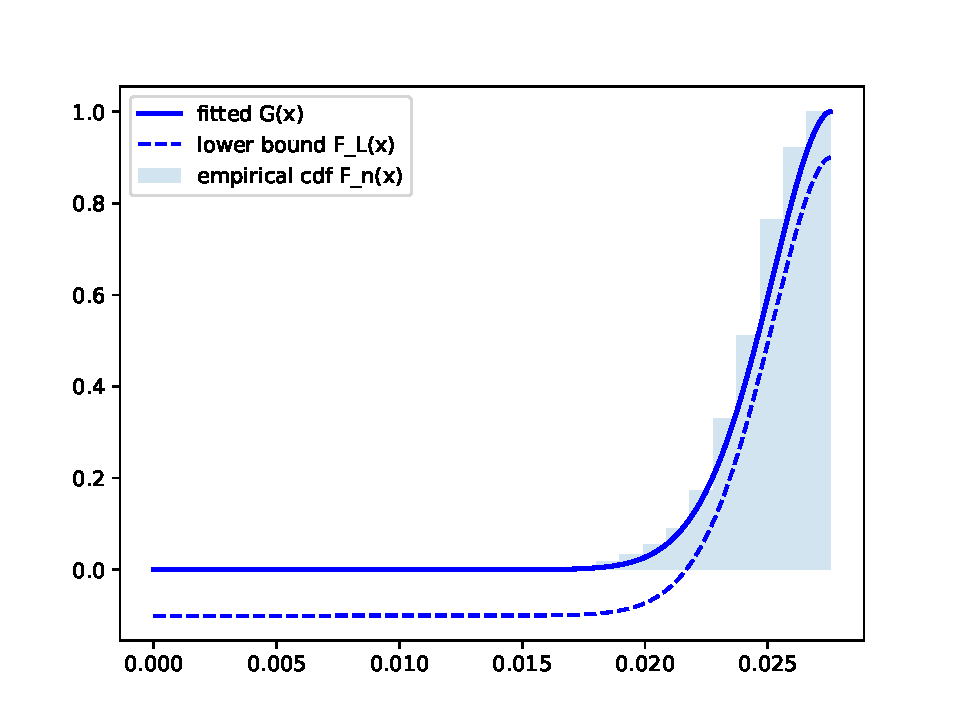
\includegraphics[width=0.48\textwidth]{images/Lemma1.pdf}
    \caption{Visualisation of the stochastic lower bound $F_{L,\gamma}$ of Lemma~\ref{app_lemma:F_L}.}
    \label{app_fig:lemma1}
\end{figure}
%
\begin{theorem}[Radius of Stochastic Lipschitz Caps]\label{app_thm:lipschitz cap}
    Given a continuous-depth model $f$ from Eq.~(1) in the main paper ($\partial_t x\,{=}\,f(x)$ with $x(t_0)\,{\in}\,\,B(x_0, \rd_0)$), $\gamma\,{\in}\,(0,1)$, $\mu\,{>}\,1$, target time $t_j$,
    % a sample point $x$, the corresponding stretching factor $\lambda_x = \|\partial_x\chi(t_j,x)\|$,
    the set of all sampled points $\calV$, the number of sampled points $N\,{=}\,|\calV|$, the sample maximum $\bar{m}_{j,\calV}\,{=}\,\max_{x\in\calV} d_j(x)$, the IVP solutions $\chi(t_j,x)$, and the corresponding stretching factors $\lambda_x\,{=}\,\|\partial_x\chi(t_j,x)\|$ for all $x\,{\in}\,\calV$. Let us define $\hat{\gamma} = 1-\sqrt{1-\gamma}$.
    Let $\Delta\lambda_{\calV}$ be the $\sqrt{1-\gamma}$-quantile of a stochastic lower bound $F_{L,\hat{\gamma}}$ as defined in Eq.~\eqref{app_eq:F_L bound} of Lemma~\ref{app_lemma:F_L}:
    \begin{align}\label{app_eq:expected difference quotient}
        \Delta\lambda_{\calV}(\gamma) = F_{L,\hat{\gamma}}^{-1}(\sqrt{1-\gamma}),
    \end{align}
    Let $r_x$ be defined as:
    \begin{align}\label{app_eq:cap radius}
        r_{x} = \frac{\left(-\lambda_x + \sqrt{\lambda_x^2 + 4\cdot\Delta\lambda_{x,\calV}\cdot(\mu\cdot\bar{m}_{j,\calV}-d_j(x))}\right)}{2\cdot\Delta\lambda_{x,\calV}},
    \end{align}
    then it holds that:
    \begin{align}\label{app_eq:cap probability}
        \Pr\left(d_j(y) \le \mu\cdot \bar{m}_{j,\calV}\right)\ge 1-\gamma\quad \forall y\in B(x,r_x)^S,
    \end{align}
    and thus that $B(x, r_x)^S$ is a $\gamma, t_j$-Lipschitz cap.
\end{theorem}
\emph{Proof.} Let $\{x_1,\dots,x_n\}$ be $n$ independent experiments by sampling from $X\,{=}\,\max_{i=1}^m|\lambda_{a_i}\,{-}\,\lambda_{b_i}|/\|a_i\,{-}\,b_i\|$ as defined in Lemma~\ref{app_lemma:F_L}, where each variable is the maximum of $m$ executions. 
From Eq.~\eqref{app_eq:prob F_L bound} it follows that:
\begin{align}\label{app_eq:cdf bound}
    Pr(F_{L,\hat{\gamma}(x)} \le F(x))\ge 1-\hat{\gamma} = \sqrt{1-\gamma}
\end{align}
Let us now derive the probability of $X$ being less or equal to $\Delta\lambda_{\calV}$ defined by Eq.~\eqref{app_eq:expected difference quotient}. 
For any sets $A, B$ it holds that $\Pr(A)\ge \Pr(A\cap B) = \Pr(A | B) \cdot \Pr(B)$, thus:
\begin{align}
    &Pr(X \le \Delta\lambda_{\calV}) \ge\\
    &\ge Pr\Big(X\le\Delta\lambda_{\calV} | F_{L,\hat{\gamma}(x)} \le F(x)\Big)\cdot\label{app_eq:quantile1}\\
    &\qquad\cdot Pr\Big(F_{L,\hat{\gamma}(x)} \le F(x)\Big)
\end{align}
Let us have a look on Eq.~\eqref{app_eq:quantile1}: As $Pr(X\le \Delta\lambda)=F(\Delta\lambda)$ and we are looking for the conditional probability depending on $F_{L,\hat{\gamma}(x)} \le F(x)$, we can use $F_{L,\hat{\gamma}}(\Delta\lambda)$ as a lower bound of Eq.~\eqref{app_eq:quantile1} and thus, using Eq.~\eqref{app_eq:cdf bound}:
\begin{align}
    Pr(X\le \Delta\lambda_{\calV}) \ge F_{L,\hat{\gamma}}(\Delta\lambda_{\calV})\cdot \sqrt{1-\gamma}
\end{align}
As Eq.~\eqref{app_eq:expected difference quotient} defines $\Delta\lambda_{\calV}$ as the $\sqrt{1-\gamma}$-quantile of $F_{L,\gamma}$, we can further state that
\begin{align}\label{app_eq:confidence lipschitz max}
    \begin{split}
    \Pr(X \le \Delta\lambda_{\calV})\ge 1-\gamma, \\\quad \textrm{with}\quad X=\max_{i=1}^m\left[\frac{|\lambda_{a_i} -  \lambda_{b_i}|}{\|a_i-b_i\|}\right]
    \end{split}
\end{align}
Let $Y\,=\, |\lambda_a-\lambda_b|/\|a-b\|$ be another random variable with $a, b$ being to sample points of the initial ball $\calB_0$. From Eq.~\eqref{app_eq:confidence lipschitz max} it holds that
\begin{align}\label{app_eq:confidence lipschitz}
    Pr(Y\le \Delta\lambda_\calV)\ge Pr(X\le \Delta\lambda_\calV)\ge 1-\gamma
\end{align}
It trivially holds for $x, y \in \calV$ that:
\begin{align}
    \lambda_y &= \lambda_x + \frac{\lambda_y - \lambda_x}{\|x-y\|}\cdot \|x-y\|\nonumber\\
    &\le \lambda_x + \frac{|\lambda_x - \lambda_y|}{\|x-y\|}\cdot \|x-y\|%,\\
    % &\le \lambda_x + \max_{x,y \in \calB_0}\frac{|\lambda_x - \lambda_y|}{\|x-y\|}\cdot \|x-y\|
\end{align}
From Eq.~\eqref{app_eq:confidence lipschitz} it follows that:
\begin{align}
    &Pr\Bigg(\lambda_x + \frac{|\lambda_x - \lambda_y|}{\|x-y\|}\cdot \|x-y\| \le \\
    &\qquad\le \lambda_x + \Delta\lambda_{x,\calV}\cdot \|x-y\|\Bigg)\ge 1-\gamma
\end{align}
and using the monotony of the probability measure:
\begin{align}
    \Pr\big(\lambda_y &\le \lambda_x + \Delta\lambda_{x,\calV}\cdot \|x-y\|\big) \ge 1-\gamma\label{app_eq:confidence bound}
\end{align}
Using the mean value inequality for vector-valued functions it holds that:
\begin{align*}
    & |d_j(x) - d_j(y)|= | \left\lVert \chi(t_j,x) - \chi(t_j,x_0)\right\rVert -\\ &\quad- \left\lVert \chi(t_j,y) - \chi(t_j,x_0)\right\rVert|\quad \textrm{\{triangle inequality\}}\\
    &\quad \le \|\chi(t_j,x) - \chi(t_j,y)\|\quad \textrm{\{mean value theorem\}}\\
    &\Rightarrow\exists z\in [x,y] \colon  |d_j(x) - d_j(y)|\\ &\quad\le \|\partial_x \chi(t_j,z) \| \|x-y\| = \lambda_z \cdot \|x-y\|
\end{align*}
Combining this with Eq.~\eqref{app_eq:confidence bound} and thus using $\lambda_x + \Delta\lambda_{x,\calV}\cdot \|x-y\|$ as a probabilistic upper bound for $\lambda_z$, we obtain the following results for all $y$ with $\|x-y\| \le r_x$:
\begin{align}
    &\Pr\big(|d_j(x)-d_j(y)|\le\nonumber\\
    &\quad\le (\lambda_x + \Delta\lambda_{x,\calV}\cdot \|x-y\|) \cdot \|x-y\|\big) \ge 1-\gamma \nonumber\\
    \begin{split}
    &\Pr\big(|d_j(x)-d_j(y)|\le\\
    &\quad\le (\lambda_x + \Delta\lambda_{x,\calV}\cdot r_x) \cdot r_x\big) \ge 1-\gamma
    \end{split}
\end{align}
As $r_x$ defined like in Eq.~\eqref{app_eq:cap radius} is the solution of the quadratic equation $\mu\cdot\bar{m}_{j,\calV}-d_j(x)=\lambda_x r_x + \Delta\lambda_{x,\calV} r_x^2$, it holds that:
\begin{align}
\begin{split}
    &\Pr\big(|d_j(x) - d_j(y)| \le \mu\cdot\bar{m}_{j,\calV}-d_j(x))\big) \ge\\
    &\quad \ge 1-\gamma \quad\forall y\in B(x, r_x)^S\label{app_eq:probabilistic lipschitz}
\end{split}
\end{align}
We now distinguish between two cases for $y$: (a)~$d_j(y)\le d_j(x)$ and (b)~$d_j(y) \ge d_j(x)$. In case (a) it is trivial: $d_j(y) \le d_j(x) \le \mu \cdot \bar{m}_{j,\calV}$. Having case (b), Eq.~\eqref{app_eq:probabilistic lipschitz} is equivalent to
\begin{align}
    \Pr\big(d_j(y) - d_j(x) &\le \mu\cdot\bar{m}_{j,\calV}-d_j(x))\big) \ge 1-\gamma\nonumber\\ &\Longleftrightarrow\nonumber\\
    \Pr\big(d_j(y) &\le \mu\cdot\bar{m}_{j,\calV})\big) \ge 1-\gamma,
\end{align}
thus Eq.~\eqref{app_eq:cap probability} holds and $B(x,r_x)^S$ is a Lipschitz cap.

\begin{theorem}[Convergence via Lipschitz Caps]\label{app_thm:stochastic guarantee} Given the tightness factor $\mu > 1$, the set of all sampled points $\calV$ and the sample maximum $\bar{m}_{j,\calV} = \max_{x\in\calV} d_j(x)$. Let the initial ball maximum be defined by $m^\star_j=\max_{x\in\calB_0} d_j(x)$. Then:
    \begin{align}\label{app_eq:stochastic guarantee}
        \hspace*{-2ex}\forall\gamma\in(0,1),\exists N\in\mathbb{N}\textrm{ s.t. }
        \Pr(\mu\cdot\bar{m}_{j,\calV}\ge m^\star_j) \ge 1-\gamma
    \end{align}
    where $N=|\calV|$ is the number of sampled points.
\end{theorem}
\emph{Proof.} Let $x^\star_j$ be a point such that $d_j(x^\star_j) = m^\star_j$. Given $\gamma\in(0,1)$ and cap radii $r_x$ as defined in Eq.~\eqref{app_eq:cap radius}, we know from the definition of a spherical cap that
\begin{align}
    &p_{r_x} = \Pr(B(x, r_x)^S\owns x_j^\star) = \frac{\area(B(x, r_x)^S)}{\area{(\calB_0})}\\
    &\textrm{and thus it holds that:}\nonumber\\
    &\Pr(\exists y\in\calV\colon B(y, r_y)^S\owns x_j^\star) = 1 - \prod_{x\in\calV} \left(
        1 - p_{r_x}
        \right)
\end{align}
We derive a lower bound of $r_x$ by using the first sample $x_{j,1}$ and replacing the values in Eq.~\eqref{app_eq:cap radius} as follows:
\begin{align}
    &\mu\cdot \bar{m}_{j,\calV} - d_j(x) \\
    &\quad\ge \mu\cdot \bar{m}_{j,\calV} - \bar{m}_{j,\calV} = (\mu - 1)\cdot \bar{m}_{j,\calV} \\
    &\quad\ge (\mu - 1) \cdot d_j(x_{j,1}),
\end{align}
thus a lower bound of all Lipschitz cap radii is given by
\begin{align}
    & r_{bound} = \nonumber\\
    &\quad=\frac{-\lambda_x + \sqrt{\lambda_x^2 + 4\cdot\Delta\lambda_{x,\calV}\cdot(\mu - 1) \cdot d_j(x_{j,1})}}{2\cdot\Delta\lambda_{x,\calV}} \le \nonumber\\
    &\quad\le r_x \quad\forall x\in \calV\nonumber\\
    \begin{split}
    &\Rightarrow \Pr(\exists y\in\calV\colon B(y, r_y)^S\owns x_j^\star) \ge \\
    &\quad\ge 1 - \left(
        1 - p_{r_{bound}}
        \right)^N\label{app_eq:lower bound probability}
    \end{split}
\end{align}
As in the limit of $N\rightarrow \infty$ the probability of Eq.~\eqref{app_eq:lower bound probability} is 1, it follows that $\forall \gamma\in (0,1)~\exists N \in\mathbb{N}\colon\Pr(\exists x\in\calV\colon\,B(x,r_x)^S\owns x^\star_j)\ge\sqrt{1-\gamma}$.

Using a set of sampled points $\calV$ with cardinality $N$ and using $\hat{\gamma} = 1-\sqrt{1-\gamma}$ as the error rate for the upper bound $\Delta\lambda_x$ of the confidence interval in Eq.~\eqref{app_eq:expected difference quotient}. Using the result of Theorem~\ref{app_thm:lipschitz cap}, the resulting probability $\forall y\in B(x,r_x)^S$ is:
\begin{align}\label{app_eq:proof lipschitz cap}
    \Pr\left(d_j(y) \le \mu\cdot \bar{m}_{j,\calV}\right)\ge 1-\hat{\gamma} = \sqrt{1-\gamma}
\end{align}
If there is an $x\in\calV$ such that $B(x,r_x)^S\owns x_j^\star$, then Eq.~\eqref{app_eq:proof lipschitz cap} obviously holds also for $x_j^\star$, thus:
\begin{align*}
    \Pr( d_j(x^\star) \le \mu\cdot\bar{m}_{j,\calV} |\exists x\in\calV\colon B(x,r_x)^S\owns x^\star)\ge \sqrt{1-\gamma}
\end{align*}
For any sets $A, B$ it holds that $\Pr(A)\ge \Pr(A\cap B) = \Pr(A | B) \cdot \Pr(B)$, and using:
\begin{align}
    A &= (\mu\cdot\bar{m}_{j,\calV}\ge m^\star_j)\\
    B &= (\exists x\in\calV\colon B(x,r_x)^S\owns x_j^\star)
\end{align}
it follows that $\Pr(\mu\cdot\bar{m}_{j,\calV}\ge m^\star_j)\ge \Pr(A|B) \cdot \Pr(B) = 1-\gamma$ and therefore Eq.~\eqref{app_eq:stochastic guarantee} holds.


%%
% https://en.wikipedia.org/wiki/Fisher–Tippett–Gnedenko_theorem
% https://en.wikipedia.org/wiki/Confidence_and_prediction_bands
% https://projecteuclid.org/journals/annals-of-probability/volume-18/issue-3/The-Tight-Constant-in-the-Dvoretzky-Kiefer-Wolfowitz-Inequality/10.1214/aop/1176990746.full
% https://projecteuclid.org/journals/annals-of-mathematical-statistics/volume-27/issue-3/Asymptotic-Minimax-Character-of-the-Sample-Distribution-Function-and-of/10.1214/aoms/1177728174.full
% https://en.wikipedia.org/wiki/Empirical_distribution_function
% https://en.wikipedia.org/wiki/Binomial_proportion_confidence_interval
% https://en.wikipedia.org/wiki/CDF-based_nonparametric_confidence_interval
% https://en.wikipedia.org/wiki/Confidence_and_prediction_bands
% https://en.wikipedia.org/wiki/Dvoretzky–Kiefer–Wolfowitz_inequality#cite_note-Massart-2
% https://en.wikipedia.org/wiki/Kolmogorov–Smirnov_test
% https://docs.scipy.org/doc/scipy/reference/generated/scipy.stats.ksone.html
% https://docs.scipy.org/doc/scipy/reference/generated/scipy.stats.kstest.html?highlight=kstest#scipy.stats.kstest
% greater = D+, less = D-